\section{Sistemi Quantomeccanici}\index{Sistemi Quantomeccanici}

Gli studi dei modelli atomici, portati avanti nei primi decenni del novecento, mostrarono l'inadeguatezza della meccanica classica nella descrizione di tutti i fenomeni che avvengono alle scale atomiche. Inoltre già in precedenza alcuni fenomeni di carattere elettromagnetico erano già stati spiegati teoricamente introducendo alcune ipotesi in contrasto con la descrizione dell'elettromagnetismo di Maxwell. Nella fattispecie Einstein mostrò che l'effetto \emph{fotoelettrico} è spiegabile teoricamente supponendo che la luce sia formata da pacchetti discreti ognuno di energia fissata e dipendente dalla frequenza dell'onda luminosa a cui appartengono secondo la relazione:
\begin{equation}
    E=h\nu\qquad\qquad\qquad h=\text{costante di Plack}. \label{relazione Planck}
\end{equation}  
Questi pacchetti discreti o quanti di luce furono in seguito chiamati \emph{fotoni} e non vi è modo di dedurre teoricamente l'ipotesi della loro esistenza dalla teoria di Maxwell. È possibile conciliare questa interpretazione con l'elettromagnetismo classico supponendo che la natura indipendente dalla frequenza dell'energia di un'onda elettromagnetica sia dovuta al fatto che: dati due fasci di luce monocromatica di eguale frequenza ma con intensità differenti il numero di fotoni che compone ogni fascio è differente ed è direttamente proporzionale all'intensità. Questa ipotesi è sperimentalmente confermata dall'effetto fotoelettrico stesso nel quale si osserva una maggior numero di fotoelettroni emessi tanto maggiore è l'intensità del fascio di luce incidente sul metallo.

\subsection{Polarizzazione di fotoni}

Una volta constatata la necessità di formulare un nuovo formalismo capace di descrivere i sistemi in cui la meccanica classica fallisce è necessario capire quali caratteristiche deve possedere questo formalismo, per farlo si consideri un sistema di fotoni che compongono un fascio di luce.\\ Per procedere è necessario avere ben presente che quanto è fisicamente possibile descrivere di un sistema è tale solamente se è possibile misurare, direttamente o indirettamente, tale proprietà e siccome senza un teoria ben sviluppata a disposizione non è ricavare grandezze non misurabili direttamente da queste sarà necessario iniziare descrivendo solamente proprietà direttamente misurabili. In questo modo non ci si domanderà come descrivere la posizione o la velocità di un fotone fin tanto non si introdurrà un sistema in grado di misurare queste.\\

Come si è già osservato nella discussione della relazione \eqref{relazione Planck} l'intensità di un fascio di luce è strettamente legata a fenomeni quantistici poiché è legata alla quantità di fotoni del fascio stesso, per questo si considererà un apparato sperimentale che consente di interagire con questa grandezza. Gli studi ottocenteschi mostrarono che un fascio di luce cambia di intensistà in seguito al passaggio attraverso alcuni filtri polarizzatori, questo secondo fatto suggerisce che può essere opportuno considerare la polarizzazione come una quantità intrinseca di ogni fotone.
\begin{figure}[H]
    \centering
    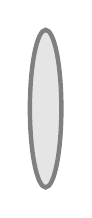
\begin{tikzpicture}
        
        \draw[ultra thick, gray, fill=black!10] (0,0) ellipse (.2 and 1);
    \end{tikzpicture}
\end{figure}
 Infatti, per quanto si è detto fin'ora, una diminuzione dell'intensità luminosa del fascio deve essere dovuta ad una diminuzione di fotoni nel fascio stesso, per cui l'interazione tra filtro e fascio è da intendersi in primo luogo come interazione tra filtro e singolo fotone che dovrà quindi essere caratterizzato anch'esso da una polarizzazione che ne determina il suo passaggio o il suo assorbimento dal filtro. Così facendo un fascio di luce polarizzato in una direzione sarà composto da soli fotoni polarizzati in tale direzione.\\
Si consideri ora un sistema di due filtri polarizzanti posti uno di seguito all'altro e tali da avere gli assi di polarizzazione reciprocamente inclinati di un angolo $\vartheta$. Un fascio di luce non polarizzata passa attraverso il primo filtro e l'elettromagnetismo classico dice che in questo passaggio la sua intensità è dimezzata, successivamente giunge al secondo filtro un fascio polarizzato totalmente nella direzione del primo filtro, questo interagendo con il secondo diminuisce di intensità secondo la \emph{legge di Malus} che da un'intensità finale pari a $(I_0 \cos^2\vartheta)/2$, dove $I_0$ è l'intensità iniziale.
\begin{figure}[H]
    \centering
    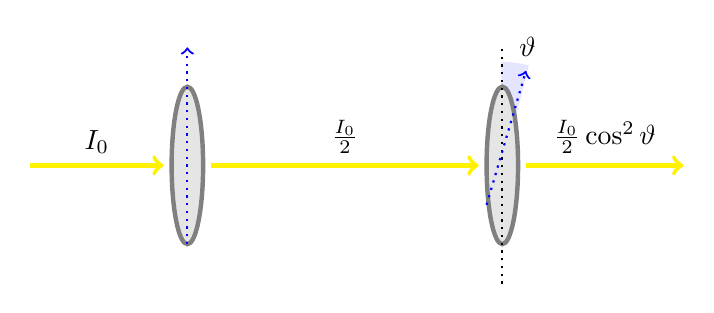
\begin{tikzpicture}
        
        \draw[ultra thick, gray, fill=black!10] (0,0) ellipse (.2 and 1);
        \draw[->,blue, dotted,thick] (0,-1)--(0,1.5);
        \draw[fill=blue!5,blue!10] (4,0) -- (4,1.3) arc(90:75:1.2369) node[anchor=south,black]{$\vartheta$} -- (4,0) ;
        \draw[ultra thick, gray, fill=black!10] (4,0) ellipse (.2 and 1);
        \draw[black, dotted,thick] (4,-1.5)--(4,1.5);
        \draw[->,blue, dotted,thick] (3.8,-.5)--(4.3,1.2);
        \draw[yellow,->,ultra thick] (-2,0) --node[anchor=south,black]{$I_0$} (-0.3,0);      
        \draw[yellow,->,ultra thick] (0.3,0) --node[anchor=south,black]{$\frac{I_0}{2}$} (3.7,0);   
        \draw[yellow,->,ultra thick] (4.3,0) --node[anchor=south,black]{$\frac{I_0}{2}\cos^2\vartheta$} (6.3,0); 
          
    \end{tikzpicture}
\end{figure}
Studiando il sistema dal punto di vista di un fotone quello che avviene è che il primo filtro lascia passare solamente i fotoni polarizzati nella sua direzione così che il fascio che giunge al secondo filtro sia polarizzato linearmente in una direzione. Per quanto detto fino ad ora il secondo filtro non dovrebbe far passare alcun fotone poiché tutti hanno una polarizzazione differente da quella di questo filtro ma ne l'elettromagnetismo classico ne l'esperienza concordano con questa interpretazione.\\ Si consideri ora un fascio con intensità tale da far passare nel sistema di filtri un solo fotone alla volta\footnote{Affinché sia soddisfatta questa condizione l'intensità del fascio deve essere dell'ordine di grandezza dell'energia di un solo fotone.}: osservazioni sperimentali mostrarono che anche in questo caso la frazione di fotoni che passano attraverso ad entrambi i filtri non è nulla ma è proporzionale all'intensità prevista dalla legge di Malus. Inoltre i fotoni che hanno attraversato entrambi i filtri hanno una polarizzazione finale differente da quella che possedevano inizialmente e dopo il passaggio attraverso il primo filtro. Tutte queste osservazioni suggeriscono che non sia possibile interpretare in maniera deterministica questo fenomeno ma è concesso solamente avere risultati teorici di natura probabilistica; l'interazione tra fotone e filtro modifica stocasticamente lo stato del fotone.\\
Così facendo inizialmente il fotone non ha una polarizzazione ben definita e interagendo con il primo filtro è forzato ad assumere una polarizzazione precisa, per le proprietà intrinseche dell'interazione, o quella del filtro o quella perpendicolare a questa. Siccome la polarizzazione iniziale non è definita è verosimile assumere che in media metà dei fotoni assumerà la polarizzazione del filtro, passandoci attraverso, e l'altra metà quella perpendicolare, venendo così assorbita. Questo approccio non spiega comunque l'interazione con il secondo filtro che può essere spiegata solamente dal \emph{principio di sovrapposizione}. Questo principio afferma che lo stato di un sistema quantistico può essere dato dalla sovrapposizione di più stati che può assumere il sistema, in questo modo si ha:
\begin{itemize}
    \item se $\vartheta=0$ il fotone uscente dal primo filtro è polarizzato in maniera da attraversare il secondo,
    \item se $\vartheta=90^\circ$ il fotone uscente nel primo filtro è polarizzato ortogonalmente al'asse del secondo filtro che quindi lo assorbe senza che esso possa passare,
    \item infine se $\vartheta\neq0$ e $\vartheta\neq90^\circ$ il fotone uscente dal primo filtro è in uno stato di sovrapposizione dei due stati precedenti e interagendo con il secondo filtro può stocatiscamente essere assorbito o trasmesso con probabilità date dalla legge di Malus.
\end{itemize}
\subsection{Interferenza di un fotone}
Si studierà ora un secondo esperimento che consente di studiare come proprietà dello stato del fotone la sua posizione, è quindi necessario costruire un apparato che consenta di misurare tale grandezza, tale sistema è costituito da una lastra fotografica che in seguito all'impatto di un fotone su di essa si impressiona nel punto in cui esso ha impattato determinandone la posizione. Questo apparato costringe quindi i fotoni ad assumere uno stato di posizione ben definita se questa non lo fosse in precedenza.\\

L'ottica classica già aveva scoperto che, interpretando la luce come un'onda, se posto uno schermo con due fenditure piccole e vicine tra una sorgente monocromatica e la lastra fotosensibile, su quest'ultima si osserva un'immagine nota come pattern di interferenza. 
\begin{figure}[H]
    \centering

    \tikzset{every picture/.style={line width=0.75pt}} %set default line width to 0.75pt        

    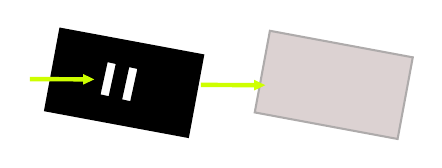
\begin{tikzpicture}[x=0.75pt,y=0.75pt,yscale=-1,xscale=1]
    %uncomment if require: \path (0,300); %set diagram left start at 0, and has height of 300
    
    %Shape: Rectangle [id:dp41952196134001873] 
    \draw  [color={rgb, 255:red, 174; green, 171; blue, 171 }  ,draw opacity=1 ][fill={rgb, 255:red, 220; green, 210; blue, 210 }  ,fill opacity=1 ] (433.24,112.94) -- (502.07,125.73) -- (494.76,165.06) -- (425.93,152.27) -- cycle ;
    %Shape: Rectangle [id:dp7509317736279448] 
    \draw  [fill={rgb, 255:red, 0; green, 0; blue, 0 }  ,fill opacity=1 ] (332.24,111.94) -- (401.07,124.73) -- (393.76,164.06) -- (324.93,151.27) -- cycle ;
    %Shape: Rectangle [id:dp5923354100874827] 
    \draw  [fill={rgb, 255:red, 255; green, 255; blue, 255 }  ,fill opacity=1 ] (354.67,127.46) -- (359.55,128.53) -- (355.93,145.04) -- (351.05,143.97) -- cycle ;
    %Shape: Rectangle [id:dp29981974919016974] 
    \draw  [fill={rgb, 255:red, 255; green, 255; blue, 255 }  ,fill opacity=1 ] (365.07,129.86) -- (369.95,130.93) -- (366.33,147.44) -- (361.45,146.37) -- cycle ;
    %Straight Lines [id:da1953558429893636] 
    \draw [ultra thick, color={rgb, 255:red, 206; green, 255; blue, 0 }  ,draw opacity=1 ][fill={rgb, 255:red, 237; green, 255; blue, 0 }  ,fill opacity=1 ]   (317.6,136.2) -- (345.6,136.34) ;
    \draw [shift={(348.6,136.36)}, rotate = 180.3] [fill={rgb, 255:red, 206; green, 255; blue, 0 }  ,fill opacity=1 ][line width=0.08]  [draw opacity=0] (5.36,-2.57) -- (0,0) -- (5.36,2.57) -- cycle    ;
    %Straight Lines [id:da061436218469033355] 
    \draw [ultra thick,color={rgb, 255:red, 206; green, 255; blue, 0 }  ,draw opacity=1 ][fill={rgb, 255:red, 237; green, 255; blue, 0 }  ,fill opacity=1 ]   (400,139) -- (428,139.14) ;
    \draw [shift={(431,139.16)}, rotate = 180.3] [fill={rgb, 255:red, 206; green, 255; blue, 0 }  ,fill opacity=1 ][line width=0.08]  [draw opacity=0] (5.36,-2.57) -- (0,0) -- (5.36,2.57) -- cycle    ;
    
    
    
    
    \end{tikzpicture}
    
\end{figure}    

Questo fatto, confermato sperimentalmente, è di difficile interpretazione con l'approccio di Einstein che considera la luce formata da fotoni. In prima istanza si potrebbe considerare che i vari fotoni passando attraverso una fenditura interferisca con quelli passanti per l'altra generando il pattern. In realtà però se si compie il medesimo esperimento facendo passare un solo fotone alla volta osservando la figura che si produce dopo aver fatto passare molti fotoni si osserva nuovamente il pattern, per cui in realtà il fenomeno osservato non è dato dall'interferenza tra fotoni ma è un fenomeno intrinseco del singolo fotone.\\ Il principio di sovrapposizione in questo caso consente di affermare che il fotone, dopo aver attraversato le due fenditure, è in una sovrapposizione di due stati: uno nel quale è passato attraverso una fenditura e uno nel quale è passato nell'altra. In questo modo sono questi due stati contemporaneamente esistenti che interferiscono tra di loro.\\

Questo esperimento mette in luce un altro aspetto fondamentale di questi fenomeni: infatti classicamente è la funzione d'onda del campo elettromagnetico che descrive il fascio di luce e il pattern di interferenza è descritto dall'intensità dell'onda che è proporzionale al modulo quadrato della funzione d'onda del fascio. Secondo l'interpretazione quantistica che si sta costruendo invece il pattern di interferenza descrive le natura probabilistica del sistema, essendo questa data però dalla funzione d'onda del fascio è naturale porre questa come stato del sistema il cui modulo quadro stima la probabilità di misurare un fotone in un punto. 

\subsection{Principio di Sovrapposizione}
Terminate le osservazioni di carattere sperimentale è necessario costruire un formalismo matematico che tenga conto di quanto precedentemente osservato.\\
Lo stato di un sistema, come si è visto, ha proprietà vettoriali, ossia può essere combinato linearmente con altri stati per ottenere ulteriori stati, questo di fatto già racchiude il principio di sovrapposizione.
\begin{definition}[Stato di un sistema]
    Lo stato di un sistema caratterizzato da grandezze $\alpha_1\ ...\ \alpha_n$ è rappresentato da un vettore \emph{ket} $\ket{\alpha_1\ ...\ \alpha_n}$.\\L'insieme di questi stati forma uno spazio vettoriale.
\end{definition}
È fondamentale osservare che la somma di due stati identici non genera un nuovo stato del sistema, infatti se la somma di due funzioni d'onda classiche varierebbero l'intensità del fascio di luce essendo questa legata solamente al numero di fotoni non variando lo stato del singolo fotone. Questo significa che eventuali fattori moltiplicativi di un singolo stato non influiscono su questo. La questione è differente se si considera la sovrapposizione di più stati $c_1\ket{\alpha}+c_2\ket{\beta}$: in questo caso vale ancora che multipli dello stato risultante rappresentano il medesimo stato di partenza ma questo non vale se si cambiano i singoli valori di $c_1$ e $c_2$. Lo stato risultante è quindi determinato dal rapporto $c_1/c_2$: si osservi che però lo stato di un fotone non in generale è determinato da un solo parametro, infatti si è visto che lo stato di un fotone è descritto dalla sua funzione d'onda del campo elettromagnetico ma la combinazione di due di queste è in ogni istante determinata sia dal rapporto dei moduli delle loro ampiezze d'onda sia da un fattore di fase. Questa osservazione mostra che i fattore $c_1$ e $c_2$ debbano essere numeri complessi e non reali, così che il loro rapporti goda di due gradi di libertà. La polarizzazione di un fotone è un chiaro esempio fisico di questa necessità infatti polarizzazioni ellittiche sono determinate sia dal rapporto delle ampiezze delle funzioni d'onda scalari di due componenti ortogonali di campo elettrico o magnetico sia dalla loro differenza di fase.\\

Poiché le costanti delle combinazioni lineari di stati, come si è appena osservato, sono parte integrante della descrizione dello stato risultante da tale combinazione è naturale dotare di un prodotto scalare lo spazio vettoriale degli stati, in modo tale da poter interagire con queste costanti.
\begin{definition}[Prodotto scalare]
    Sia $\braket{\alpha |\beta}$ un applicazione che associa a due vettori $\ket{\alpha}$ e $\ket{\beta}$ un numero complesso. Si dirà tale applicazione prodotto scalare se:
    \begin{itemize}
        \item è lineare rispetto a $\ket{\beta}$ e antilineare rispetto $\ket{\alpha}$,
        \item $\braket{\alpha |\beta}=\overline{\braket{\beta |\alpha}}$, dove con $\bar z$ si intende il complesso coniugato di $z$,
        \item $\braket{\alpha |\alpha}\geq0$ per ogni $\ket{\alpha}$ a meno che $\ket{\alpha}=0$ per cui $\braket{\alpha |\alpha}=0$.
    \end{itemize} 
\end{definition}
Il teorema di rappresentazione di Riesz consente, una volta definito un prodotto scalare e fissato un vettore ket $\ket{\alpha}$, di identificare univocamente un'applicazione lineare tale che $\varphi_{\alpha}(\ket{\beta})=\braket{\alpha |\beta}$. Questa applicazione appartiene allo spazio duale dello spazio degli stati: in virtù di questo del fatto che il duale di uno spazio vettoriale è a sua volta uno spazio vettoriale si chiamano i duali degli stati vettori \emph{bra} $\bra{\alpha}=\varphi_{\alpha}$.\\
Il prodotto scalare così introdotto consente di calcolare la norma di uno stato così da operare l'operazione di \emph{normalizzazione}, questa poiché, come si è osservato, lo stato del sistema è definito a meno di fattori moltiplicativi e in seguito si rivelerà utile fare uso di questi vettori normalizzati.\\
Infine è importante definire, in analogia geometrica, cosa siano due vettore ortogonali.
\begin{definition}
    Si diranno $\ket{\alpha}$ e $\ket{\beta}$ ortogonali se e solo se $\braket{\alpha |\beta}=0$.
\end{definition}
Se ora si considerando due vettori normalizzati e ortogonali $\ket{\alpha}$ e $\ket{\beta}$, la cui combinazione lineare da luogo allo stato $\ket{\gamma}$, si ha che $\braket{\alpha|\gamma}$ è proprio il coefficiente di $\ket{\alpha}$ nella combinazione lineare.
\section{Osservabili di un sistema}
\subsection{Osservabili e operatori lineari}
Ora che si è definito il formalismo con cui descrivere uno stato è necessario descrivere matematicamente come da tale stato sia possibile ottenere le quantità misurabili sperimentalmente, ossia gli osservabili. Inoltre si vuole poter definire questi osservabili in analogia con quelli classici e in maniera tale che si comportino similmente a questi. \\Per poter capire come ottenere gli osservabili è necessario fare un'ipotesi generale ma anche di buon senso: come si è visto tramite prodotti scalari, ossia particolari operatori lineari, è possibile ottenere le informazioni determinanti sullo stato di sovrapposizione del sistema, ossia i coefficienti delle sovrapposizioni, è quindi sensato supporre che siano sempre altri operatori lineari, o più in generale combinazioni di questi, a permettere di ottenere gli osservabili caratteristici dello stato.\\ 

Si consideri l'esperimento di polarizzazione della luce, all'interazione tra filtro e fotone si associa un operatore $\hat Q$ e allo stato del fotone il vettore $\ket{\alpha}$: si consideri in primo luogo il fotone polarizzato come il filtro, si osserva quindi che questi due interagiscono e il fotone finale è ancora nel suo stato iniziale, si può dire che $\hat Q\ket{\alpha}=\ket\alpha$, viceversa se la polarizzazione del fotone è perpendicolare a quella del filtro si ha $\hat Q\ket{\alpha}=0$ per indicare che il fotone è stato assorbito. Questa considerazione suggerisce che il valore dell'osservabile è rappresentato dagli autovalori dell'operatore: in questo caso le due relazioni descritte esprimono due autovalori $0$ e $1$, corrispondenti agli osservabili di polarizzazione rispettivamente coincidente e normale al filtro.\\ A ognuno di questi autovalori è associato uno o più autovettori (o autoket) $\hat Q$.\\
Considerando ora un fotone con polarizzazione qualsiasi si può considerare lo stato come un sovrapposizione degli stati di polarizzatone parallela e normale a quella del filtro, si indicheranno questi due fissando i valori di $\alpha$ pari agli autovalori di $\hat Q$, così che si abbia:
\begin{equation*}
    \ket{\alpha}=c_0\ket{0}+c_1\ket{1}.
\end{equation*}
Se si applica a questo l'operatore $\hat Q$ si ottiene:
\begin{equation*}
    \hat Q\ket{\alpha}=c_0\hat Q\ket{0}+c_1\hat Q\ket{1}=c_1\ket{1},
\end{equation*}
che corrisponde a quanto osservato sperimentalmente: ossia che i fotoni, successivamente al passaggio attraverso il filtro, sono in uno stato di polarizzazione parallela al filtro.
\subsection{Operatori autoaggiunti}
In generale gli autovalori di un operatore, siccome si sta considerando uno spazio vettoriale su campo complesso come spazio degli stati, sono numeri complessi, se però questi devono rappresentare le possibili misure di un osservabile devono necessariamente essere numeri reali puri. Per questo motivo gli operatori di osservabili vengono sempre assunti essere autoaggiunti.\\
Per definire cosa significhi operatore autoaggiunto è necessario definire in primo luogo l'aggiunto di un operatore.
\begin{definition}[Aggiunto di un operatore]
    Sia $\hat{A}$ un operatore lineare allora si dirà \emph{aggiunto di $\hat{A}$} l'operatore $\hat{A}^*$ tale che:
    \begin{equation}
        \bra{\alpha}(\hat A\ket\beta)=(\hat{A}^*\bra{\alpha})\ket\beta.
    \end{equation}
\end{definition}
L'esistenza di questo operatore è data dal teorema di rappresentazione di Riesz che garantisce che esista, fissato $\ket{\alpha}$, un unico operatore lineare tale che $\varphi_{\alpha}(\ket\beta)=\bra{\alpha}(\hat A\ket\beta)$, in questo modo di $\hat{A}^*$ è costruito come l'operatore che associa a $\ket{\alpha}$ l'operatore $\varphi_{\alpha}$.
\begin{definition}[Operatore autoaggiunto]
    Sia $\hat{A}$ un operatore lineare, se vale $\hat A=\hat{A}^*$ allora è detto autoaggiunto.
\end{definition}
\begin{notation}
    Si indica il prodotto scalare $\bra{\alpha}(\hat A\ket\beta)$ con $\braket{\alpha|\hat A|\beta}$.
\end{notation}
Direttamente dalla definizione di operatore autoaggiunto si hanno alcune proprietà importanti di questi operatori. 
\begin{proposition}
    Sia $\hat A$ un operatore lineare autoaggiunto, allora la quantità $\braket{\lambda|\hat A|\lambda}\in\mathbb{R} $.\\
    Inoltre se $\ket{\lambda}$ è un suo autoket di autovalore $\lambda$ si ha che $\lambda\in\mathbb{R}$.\\Infine se $\ket{\xi}$ è un altro autoket di autovalore $\xi\neq\lambda$ allora $\braket{\xi|\lambda}=0$
\end{proposition}  
\begin{proof}
    Si osservi che essendo $\hat A$ autoaggiunto vale $\forall\ket{\lambda}$:
    \begin{equation*}
        \braket{\lambda|\hat A|\lambda}=\overline{\braket{\lambda|\hat A^*|\lambda}}=\overline{\braket{\lambda|\hat A|\lambda}},
    \end{equation*}
    questa relazione mostra che $\braket{\lambda|\hat A|\lambda}$ è pari al suo coniugato complesso per cui deve essere reale.
    Se ora $\ket{\lambda}$ è un suo autoket di autovalore $\lambda$ si ha:
    \begin{equation*}
        \braket{\lambda|\hat A|\lambda}=\braket{\lambda|\lambda}\lambda=\overline{\braket{\lambda|\hat A|\lambda}}=\overline{\braket{\lambda|\lambda}}\bar{\lambda}=\braket{\lambda|\lambda}\bar{\lambda},
    \end{equation*}
       da questa si deduce che $\lambda=\bar{\lambda}$ che deve quindi essere reale.\\
       Infine se $\ket{\xi}$ è un altro autoket di autovalore $\xi\neq\lambda$ e considerando $\braket{\lambda|\hat A|\xi}$ si ha:
       \begin{equation*}
        \braket{\lambda|\hat A|\xi}=\braket{\lambda|\xi}\xi=\overline{\braket{\xi|\hat A|\lambda}}=\overline{\braket{\xi|\lambda}}\lambda=\braket{\lambda|\hat A|\xi}\lambda,
    \end{equation*}
    segue che 
    \begin{equation*}
        \braket{\lambda|\hat A|\xi}\lambda-\braket{\lambda|\xi}\xi=\braket{\lambda|\xi}(\lambda-\xi)=0
    \end{equation*}
    ma poiché per ipotesi $\xi\neq\lambda$ allora necessariamente $\braket{\lambda|\xi}=0$.
\end{proof}
\subsection{La funzione d'onda quantistica}
Si consideri ora l'esperimento di interferenza della luce: inizialmente si fissi un punto $x$ sulla lastra fotosensibile, l'osservabile desiderato è "\emph{il moto del fotone termina in $x$?}" e a questo si associ $\hat Q_x$ con autoket $\ket{1}$, se il fotone termina in $x$, e $\ket{0}$ altrimenti. Lo stato di un fotone sarà quindi dato dalla sovrapposizione di tutti gli stati caratterizzati dal punto terminale della traiettoria: applicando $\hat Q_x$ a questo stato si otterrà quindi solamente lo stato in cui il fotone termina il moto in $x$ moltiplicato per il suo coefficiente che si chiamerà $\psi$. Facendo ora variare $x$ su tutta la lastra si ottiene una funzione di autovalori $\psi(x)$, inoltre non si potrà più parlare di autoket $\ket{1}$ ma si parlerà di autoket $\ket{x}$.\\
Chiaramente $\psi(x)$ è una funzione caratteristica dello stato dei fotoni, per questo indicheremo tale stato con $\ket{\psi}$; inoltre per costruzione, siccome questa funzione determina i coefficienti di sovrapposizione dello stato rispetto agli autoket $\ket{x}$ ed essendo tutti questi autoket ortogonali in quanto autoket di un operatore autoaggiunto, a patto di aver normalizzato tutti i $\ket{x}$, vale la seguente relazione:
\begin{equation}
    \braket{x|\psi}=\psi(x).
\end{equation} 
È plausibile supporre che la funzione $\psi(x)$ stimi la probabilità di osservare il moto terminale del fotone in $x$: infatti, alla luce delle osservazioni sulla relazione tra intensità luminosa e quantità di fotoni già fatte nelle sezioni precedenti, il pattern di interferenza che emerge dalla sovrapposizione degli stati del un fotone è da interpretare come distribuzione di probabilità della posizione finale di questo. La sovrapposizione è infatti determinata per costruizione da $\psi(x)$. Questa funzione è però a valori complessi, siccome è data dai coefficienti di sovrapposizione che sono numeri complessi, e quindi per poter essere ricondotta ad una stima della probabilità deve essere ridotta ad una funzione a valori reali. Per far ciò si può supporre che tale probabilità sia stimata dal modulo quadro di $\psi(x)$. Inoltre è necessario che questa funzione sia normalizzata ad $1$, il che può sempre essere fatto siccome ogni stato può, nel suo complesso, esser moltiplicato per uno scalare senza che questo modifichi lo stato fisico che descrive. In questo modo la probabilità di osservare un fotone in una regione dello schermo $\mathcal{D}$ è data da 
\begin{equation}
   P(\mathcal{D} )=\int_\mathcal{D} |\braket{x|\psi}|^2\ dx.
\end{equation}
Analogamente, siccome si è identificata la distribuzione di probabilità della posizione del fotone con $|\braket{x|\psi}|^2$, è possibile calcolare i momenti di questa, ossia il valor medio della posizione e la sua deviazione standard:
\begin{flalign}
    \braket{x}&=\int_\mathcal{D} x|\braket{x|\psi}|^2\ dx,\\
    \Delta x&=\sqrt{\int_\mathcal{D} (x-\braket{x})^2|\braket{x|\psi}|^2\ dx}.
\end{flalign}
In questi integrali $x$ è da intendere come un vettore di $\mathbb{R}^2$, ossia un punto del piano.\\

Infine si vuole esprimere $\ket{\psi}$ rispetto agli autoket $\ket x$, come si è detto questo è possibile tramite una sovrapposizione di questi, bisogna notare che però in questo caso gli autoket sono una quantità non numerabile, uno per ogni punto della lastra fotografica, per questo invece di un classica combinazione lineare è necessario utilizzare un'integrale:
\begin{equation}
    \ket{\psi}=\int \ket{x}\psi(x)\ dx=\int \ket{x}\braket{x|\psi}\ dx.
\end{equation}
\subsection{Basi ortonormali}